\documentclass[openany]{book}
% !TeX TXS-program:compile = txs:///pdflatex/[--shell-escape]
\usepackage{macros}
\usepackage{notes}
\usepackage{array}

%% PICTURES DIRECTORY %%

%% RENEW TITLE PAGE %%
\renewcommand{\mytitle}[2]{%
	\title{#1}
	\author{Michael Pham}
	\date{#2}
	\maketitle
	\newpage
	\mytoc
	\newpage
}

\begin{document}
\mytitle{Math 116 Pre-Studying}{Spring 2025}

\chapter{An Introduction to Cryptography}
\section{Simple Substitution Ciphers}
\subsection{Caesar (Shift) Ciphers}
To begin with, we will explore one of the most basic ciphers: the \textit{Caesar Cipher}. In this cipher, each letter in our unencrypted message (the \textit{plaintext}) gets shifted by some amount to encrypt our message (the \textit{ciphertext}). A basic example of a Caesar Cipher is seen in Example \ref{ex:1.1}.

\begin{example}[\label{ex:1.1}Basic Caesar Cipher Walkthrough]
	Suppose we had the following ciphertext:
	\begin{center}
		\texttt{j s j r d k f q q n s l g f h p g w j f p y m w t z l m n r r n s j s y q z h n z x}
	\end{center}
	
	Then, if we knew that it had been shifted up by five letters, we can apply the reverse, yielding us:
	\begin{center}
		\texttt{j s j r d k f q q n s l g f h p g w j f p y m w t z l m n r r n s j s y q z h n z x}
		\underline{\hspace{\textwidth}} \\
		\texttt{e n e m y f a l l i n g b a c k b r e a k t h r o u g h i m m i n e n t l u c i u s}
	\end{center}
	
	Then, breaking up the decrypted plaintext and breaking it into words appropriately, along with supplying the right punctuation, we get:
	\begin{center}
		\texttt{Enemy falling back. Breakthrough imminent. Lucius.}
	\end{center}
\end{example}


Now, the question may arise: what happens if the message had a letter such as \texttt{d}? There are no letters that are five before \texttt{d}. Well, in that case, we instead wrap away to the end of the alphabet.

More concretely, for \texttt{d}, it becomes \texttt{y} in our ciphertext.

A nice way to visualize the Caesar cipher then is to place the letters in our alphabet in a circle rather than a line in order to encapsulating this ``wrapping" property. This creates what we call a \textit{Cipher Wheel}, as is illustrated in Figure \ref{fig:1.1}.

Due to how the method works, Caesar Ciphers are also referred to as \textit{Shift Ciphers}. Now, an issue with the cipher arises in the following scenario:

Suppose that Alice wants to send a secret message to Bob. Using the Caesar Cipher, she encrypts her message and sends it to Bob.

However, Eve intercepts the message! The issue with this encryption method is immediately obvious: it's incredibly easy to decrypt, with Eve only needing to try out 26 shifts at most to crack the message.

The question becomes then: is there a way to make the message harder to be decrypted? One way in which Alice can do so is to use a more complicated replacement scheme.

\begin{figure}
	\begin{center}
		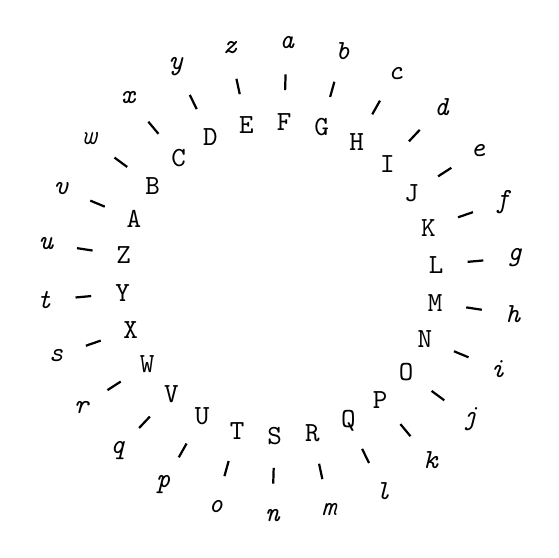
\begin{tikzpicture}
		% Circle parameters
		\def\radius{2cm}
		\foreach \i [count=\n] in {Z,...,A} {
			% Calculate angles
			\pgfmathsetmacro{\angle}{\n * (360 / 26) + 157.5} % Rotate the starting point to 12 o'clock
			%			\pgfmathsetmacro{\nextangle}{\angle + 360 / 26}
			
			% Place uppercase letters
			\node[font=\bfseries] at (\angle:\radius) {\texttt{\i}};
			
			% Place lowercase letters below uppercase letters
			\node[font=\itshape] at (\angle:\radius+1cm) {%
				\ifcase\n \or \texttt{u}\or \texttt{t}\or \texttt{s}\or \texttt{r}\or \texttt{q}\or \texttt{p}\or \texttt{o}\or \texttt{n}\or \texttt{m}\or \texttt{l}\or \texttt{k}\or \texttt{j}%
				\or \texttt{i}\or \texttt{h}\or \texttt{g}\or \texttt{f}\or \texttt{e}\or \texttt{d}\or \texttt{c}\or \texttt{b}\or \texttt{a}\or \texttt{z}\or \texttt{y}\or \texttt{x}\or \texttt{w}\or \texttt{v}\fi
			};
			
			% Draw lines connecting uppercase and lowercase letters
			\draw[thick] (\angle:\radius+0.6cm) -- (\angle:\radius+0.4cm);
		}
		\end{tikzpicture}
		\caption{Cipher Wheel with offset of 5}
		\label{fig:1.1}
	\end{center}
\end{figure}

\subsection{Simple Substitution Ciphers}
\begin{example}[\label{ex:1.2}An Alternate Scheme]
	A scheme that Alice can employ is to replace every occurrence of a letter with another one: for example, consider replacing every occurrence of \texttt{z} with \texttt{a}, and vice-versa. And then you continue with $\texttt{y} \leftrightarrow \texttt{b}, \texttt{x} \leftrightarrow \texttt{c}, \ldots, \texttt{m} \leftrightarrow \texttt{n}$.
\end{example}

This is what we call a \textit{Simple Substitution Cipher}, where each letter is replaced by another letter. In fact, the Caesar Cipher is an example of a simple substitution cipher, although many other types exist as well.

One way to view substitution ciphers is to think of them as a function $f : \brc{\texttt{a}, \ldots, \texttt{z}} \rightarrow \brc{\texttt{A}, \ldots, \texttt{Z}}$.

\begin{rmk}
	For the remainder of these notes, we will be using lowercase for the plaintext, and uppercase for the ciphertext to make it more distinguishable.
\end{rmk}

Now, for an encryption function to be valid, it must be \textit{injective} -- that is, no two plaintext letters get mapped to the same ciphertext letter.

\subsection{Cryptanalysis of Simple Substitution Ciphers}
A natural question to ask is: how many simple substitution ciphers are there?

Well, we proceed as follows to figure this out:
\begin{enumerate}
	\item First, \texttt{a} has $26$ letters it can be mapped to.
	\item Next, \texttt{b} has $25$ letters it can be mapped to.
	\item We continue until \texttt{z} which has $1$ letter it can be mapped to.
\end{enumerate}

Putting this all together, we observe then that we have:
\begin{equation*}
	26 \cdot 25 \cdots 2 \cdot 1 = 26! = 403291461126605635584000000
\end{equation*}

In other words, there are over $10^{26}$ different simple substitution ciphers. We define each associated encryption table to be a \textit{key}.

Now, suppose that Alice tries to send a message to Bob. However, Eve intercepts it and tries to decrypt it by trying every possible substitution cipher. We define \textit{Cryptanalysis} to be the process of decrypting a message without knowing the underlying key.

Now, since there are over $10^{26}$ different simple substitution ciphers, even if Eve can check one million cipher alphabets per second, it'd still take over $10^{13}$ years to crack.

However, this is where one of the most important ideas of this course comes into play:
\begin{thm}[\label{thm:1.3}Enemy Knows Best]
	The security of an encryption system depends on the \underline{best known} method to break it.
\end{thm}

Going back to simple substitution ciphers, we note that a fatal flaw exists: the English language is \textit{not} random. For example, \texttt{q} is almost always followed by \texttt{u}. Certain letters also appear more frequently than others, as seen in Figure \ref{fig:1.2}.

With that in mind, Eve can simply count the frequency of the letters in the secret message and make an educated substitution for them. Thus, the actual number of tries needed is much lower than the massive $10^{26}$.

\begin{figure}[H]
	\begin{center}
		\begin{tabular}{|l c||l c|}
			\hline
			\multicolumn{2}{|c||}{By decreasing frequency} & \multicolumn{2}{c|}{In alphabetical order} \\
			\hline
			E & 13.11\% & A & 8.15\% \\
			T & 10.47\% & B & 1.44\% \\
			A & 8.15\% & C & 2.76\% \\
			O & 8.00\% & D & 3.79\% \\
			N & 7.10\% & E & 13.11\% \\
			R & 6.83\% & F & 2.92\% \\
			I & 6.35\% & G & 1.99\% \\
			S & 6.10\% & H & 5.26\% \\
			H & 5.26\% & I & 6.35\% \\
			D & 3.79\% & J & 0.13\% \\
			L & 3.39\% & K & 0.42\% \\
			F & 2.92\% & L & 3.39\% \\
			C & 2.76\% & M & 2.54\% \\
			M & 2.54\% & N & 7.10\% \\
			U & 2.46\% & O & 8.00\% \\
			G & 1.99\% & P & 1.98\% \\
			Y & 1.98\% & Q & 0.12\% \\
			P & 1.98\% & R & 6.83\% \\
			W & 1.54\% & S & 6.10\% \\
			B & 1.44\% & T & 10.47\% \\
			V & 0.92\% & U & 2.46\% \\
			K & 0.42\% & V & 0.92\% \\
			X & 0.17\% & W & 1.54\% \\
			J & 0.13\% & X & 0.17\% \\
			Q & 0.12\% & Y & 1.98\% \\
			Z & 0.08\% & Z & 0.08\% \\
			\hline
		\end{tabular}
		\caption{Frequency of letters in English text}
		\label{fig:1.2}
	\end{center}
\end{figure}

\section{Divisibility and GCD}
In this section, we will delve into the foundations of algebra and number theory. A lot of cryptography is built on top of this.

With that in mind, we will first discuss some basic number theory -- that is, the study of integers.

To begin our discussion of the integers, $\ZZ$, we recall that they form a ring -- that is, an abelian group under $+$ and $\times$ obeys associativity, distributivity, and has a multiplicative identity $1$.

Now, with that in mind, we note that multiplication doesn't always have an inverse: that is, we can't always divide an integer by another integer. This leads to the concept of ``divisibility":

\begin{defn}[\label{def:1.5}Divisibility]
	Let $a$ and $b$ be integers such that $b \neq 0$. Then, we say that $b$ divides $a$ (or $a$ is divisible by $b$) if there exists an integer $c$ such that:
	\begin{equation*}
		a = bc
	\end{equation*}
	
	We denote this by $b \mid a$. If $b$ doesn't divide $a$, we write $b \nmid a$.
\end{defn}

\label{ex:1.6}\begin{example}
	We note that $847 \mid 485331$ as $485331 = 847 \cdot 573$.
	
	On the other hand, $355 \nmid 259943$, as when we try to divide $259943$ by $355$, we get a remainder of $83$. That is, $259943 = 355 \cdot 732 + 83$.
\end{example}

There are various divisibility properties, some of which are listed here:
\label{prop:1.7}\begin{prop}
	Let $a,b,c \in \ZZ$ be integers. Then,
	\begin{enumerate}
		\item If $a \mid b$ and $b \mid c$, then $a \mid c$.
		\item If $a \mid b$ and $b \mid a$, then $a = \pm b$.
		\item If $a \mid b$ and $a \mid c$ then $a \mid (b + c)$ and $a \mid (b - c)$.
	\end{enumerate}
\end{prop}
\begin{proof}
	Suppose that $a, b, c \in \ZZ$. Now, we will prove the first statement:
	\begin{innerproof}
		Suppose that $a \mid b$ and $b \mid c$. Then, this means that there exists $x$ and $y$ such that:
		\begin{align*}
			b &= ax \\
			c &= by \\
			&= (ax)y \\
			&= a(xy)
		\end{align*}
		
		And since $xy \in \ZZ$, we note then that exists a $z = xy \in \ZZ$ such that $c = az$; this is precisely what it means for $a \mid c$.
	\end{innerproof}
	
	Next, we prove the second statement:
	\begin{innerproof}
		Suppose that $a \mid b$ and $b \mid a$. Then, there exists $x, y$ such that:
		\begin{align*}
			b &= ax \\
			a &= by
		\end{align*}
		
		Then, this means that:
		\begin{align*}
			b &= ax \\
			&= (by)x \\
			1 &= yx
		\end{align*}
		
		Then, this means that $x = y = \pm 1$. With that in mind, we see then that $a = \pm b$ as desired.
	\end{innerproof}
	
	Finally, we prove the last statement:
	\begin{innerproof}
		Suppose that $a \mid b$ and $a \mid c$. Then, there exists $x, y \in \ZZ$ such that:
		\begin{align*}
			b &= ax \\
			c &= ay
		\end{align*}
		
		Then, we observe that:
		\begin{align*}
			b+c &= ax + ay \\
			&= a(x+y) \\
			b-c &= ax-ay \\
			&= a(x-y)
		\end{align*}
		
		Then, there exists $z_1, z_2 \in \ZZ$ such that $z_1 = x+y$ and $z_2 = x-y$ such that $az_1 = b+c$ and $az_2 = b-c$. This is precisely what it means for $a \mid (b+c)$ and $a \mid (b-c)$.
	\end{innerproof}
	
	Thus, we have proven all three properties as desired.
\end{proof}

\begin{defn}[\label{def:1.8}(Greatest) Common Divisor]
	Let $a, b \in \ZZ$. Then, we define a common divisor $d$ to be a positive integer that divides both $a$ and $b$. That is, $d \mid a$ and $d \mid b$.
	
	As its name suggests then, the Greatest Common Divisor (GCD) is the greatest $d$ such that $d \mid a$ and $d \mid b$. This is denoted by $\gcd(a,b)$.
\end{defn}


\end{document}